	
Let x be an odd natural number and y be the odd natural number consecutive to x.
	\begin{align}
	\therefore y=x+2
	\end{align}
	We need to find x and y  such that 
	\begin{multline}
x,y >10 \text{ and } x+y<40\\
\therefore x+x+2<40\\
2x+2<40\\
x+1<20\\
x<19
	\end{multline}
	
	
	Hence the condition is satisfied when $x>10$ and $x<19$
	
	
	
	The following python code computes the required pairs of consecutive odd natural numbers which satisfy the required condition, shown in Fig.\ref{fig:3.11.5_fifteen}.
	\begin{lstlisting}
	./solutions/5/codes/lines/q15.py
	\end{lstlisting}
	\begin{figure}[!ht]
	\centering
	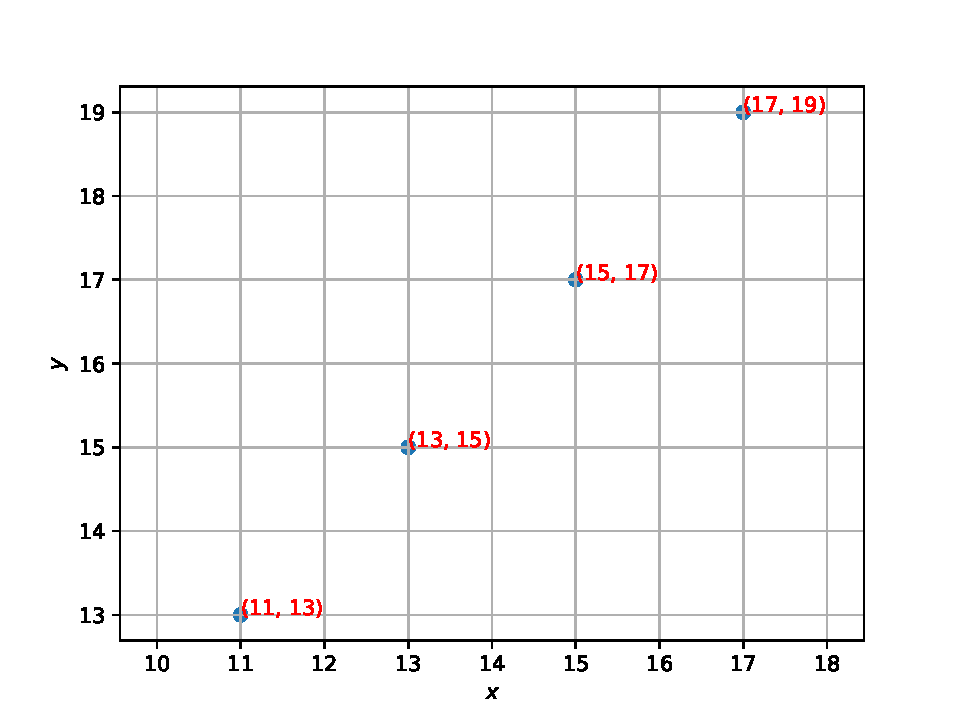
\includegraphics[width=\columnwidth]{./solutions/5/figs/lines/q15.eps}
	\caption{}
	\label{fig:3.11.5_fifteen}	
	\end{figure}
